% ============================================================
% 第15章：连续函数——一笔画
% ============================================================

\chapter{连续函数——从极限到连续}

\begin{applicationbox}
\textbf{学完本章你能做什么？}
\begin{enumerate}
  \item 理解\textbf{连续}的严格定义——极限等于函数值
  \item 能判断函数在一点处是否连续
  \item 能分类\textbf{间断点}——可去、跳跃、无穷、振荡
\end{enumerate}
\end{applicationbox}


% ============================================================
\section{从极限到连续}
% ============================================================

极限研究的是 \(x \to a\) 时 \(f(x)\) 趋近于什么——不关心 \(x=a\) 处的值。

连续则要求：\textbf{极限值等于函数值}。

\begin{definitionbox}[连续的定义]
函数 \(f\) 在 \(x=a\) 处\textbf{连续}，如果：
\[
\lim_{x \to a} f(x) = f(a)
\]

用 ε-δ 语言：对任意 \(\varepsilon > 0\)，存在 \(\delta > 0\)，
使得 \(|x-a| < \delta\) 时 \(|f(x) - f(a)| < \varepsilon\)。
\end{definitionbox}

\begin{examplebox}[1——连续 vs 间断]
\begin{center}
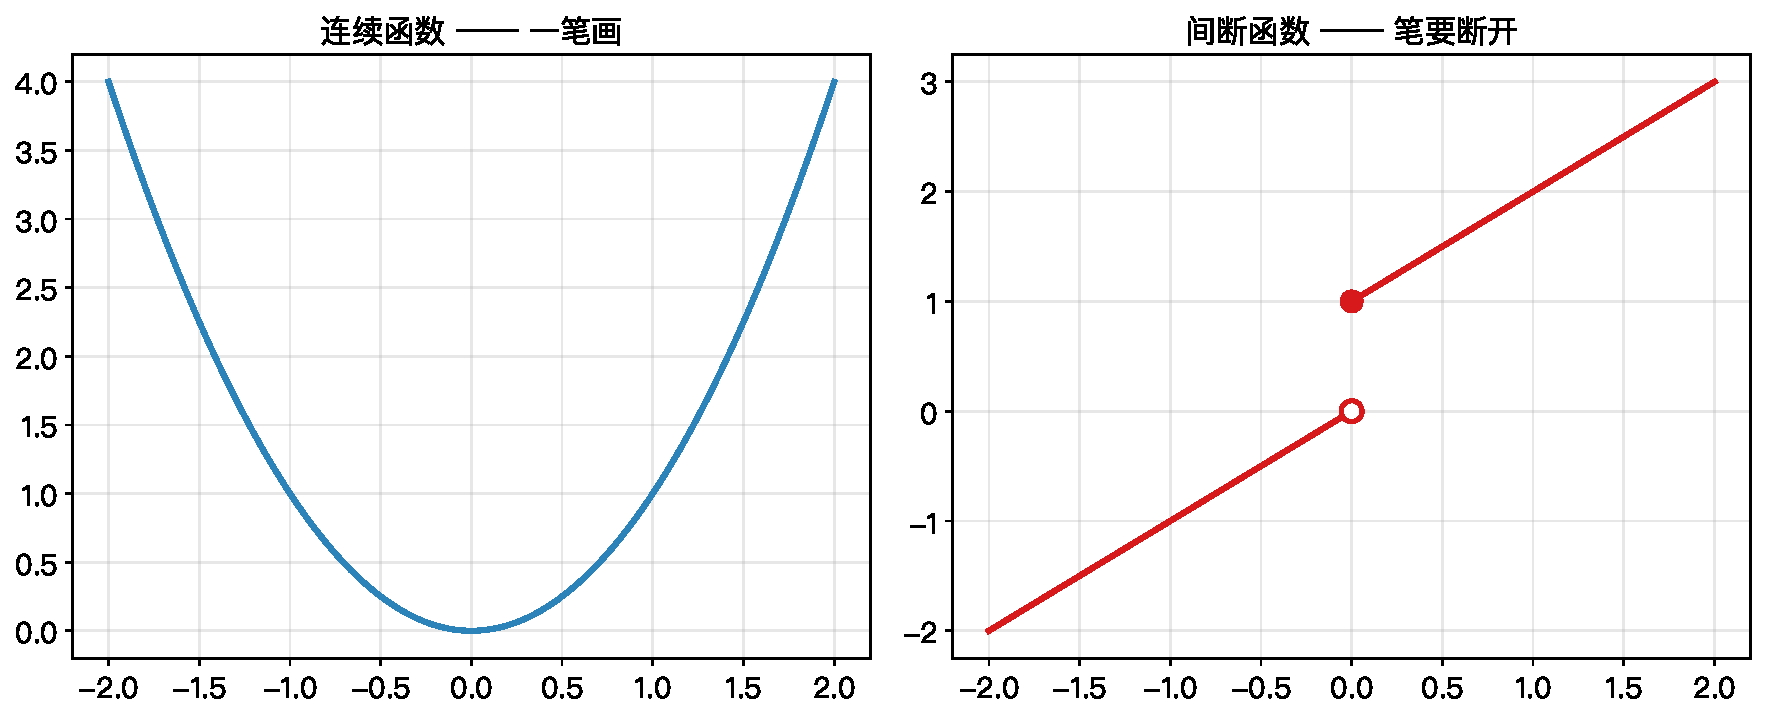
\includegraphics[width=0.85\textwidth]{figures/ch15_continuous_vs_discontinuous.pdf}
\end{center}

\textbf{左图：} \(y = x^2\)——在 \(x=0\) 处连续（\(\lim_{x\to0} x^2 = 0 = f(0)\)）\\
\textbf{右图：} 分段函数在 \(x=0\) 处间断——左右极限不等
\end{examplebox}


% ============================================================
\section{间断点的分类}
% ============================================================

\begin{definitionbox}[间断点分类]
\begin{center}
\begin{tabular}{c|c|c}
\textbf{类型} & \textbf{特征} & \textbf{例子} \\
\hline
\textbf{可去间断点} & 极限存在但不等于函数值 & \(y=\frac{x^2-1}{x-1}\) 在 \(x=1\) \\
\textbf{跳跃间断点} & 左右极限存在但不相等 & \(y=\frac{|x|}{x}\) 在 \(x=0\) \\
\textbf{无穷间断点} & 极限为无穷大 & \(y=\frac{1}{x}\) 在 \(x=0\) \\
\textbf{振荡间断点} & 极限不存在（振荡） & \(y=\sin\frac{1}{x}\) 在 \(x=0\) \\
\end{tabular}
\end{center}
\end{definitionbox}


% ============================================================
\section{本章小结}
% ============================================================

\begin{progressbox}
\textbf{连续}：\(\lim_{x\to a} f(x) = f(a)\)——极限等于函数值

\textbf{间断点}：可去、跳跃、无穷、振荡四种

初等函数在其定义域内都是连续的
\end{progressbox}


% ============================================================
\section{邻域语言——从 ε-δ 到开集}
% ============================================================

ε-δ 语言精确但繁琐。每次写"存在 δ>0 使 |x-a|<δ"很重复。
**邻域语言**把 ε-δ 的核心操作封装成更抽象的词汇。

\subsection{ε-邻域}

\begin{definitionbox}[邻域]
设 \(a\in\mathbb{R}\)，\(\varepsilon>0\)。称区间 \((a-\varepsilon, a+\varepsilon)\) 为 \(a\) 的
\textbf{ε-邻域}（读作 lín yù，英文 neighborhood），记作 \(U(a,\varepsilon)\)。

\[
U(a,\varepsilon) = \{x\in\mathbb{R}: |x-a|<\varepsilon\}
\]
\end{definitionbox}

用邻域语言翻译 ε-δ 定义：

\begin{center}
\fcolorbox{green!30}{green!5}{\parbox{0.85\textwidth}{
\(\displaystyle\lim_{x\to a}f(x)=L\) 的意思是：\\
对 \(L\) 的任意邻域 \(U(L,\varepsilon)\)，存在 \(a\) 的邻域 \(U(a,\delta)\)，
使得 \(f(U(a,\delta)\setminus\{a\}) \subseteq U(L,\varepsilon)\)。
}}
\end{center}

这比"对任意 ε>0 存在 δ>0 使得……"更紧凑，而且可以推广到高维空间。

\subsection{开集与闭集}

\begin{definitionbox}[开集与闭集]
\begin{itemize}
  \item \(U\subset\mathbb{R}\) 称为\textbf{开集}（open set），如果 \(U\) 中每一点都有一个
        完全包含在 \(U\) 内的邻域。
  \item \(F\subset\mathbb{R}\) 称为\textbf{闭集}（closed set），如果它的补集 \(\mathbb{R}\setminus F\) 是开集。
\end{itemize}
\end{definitionbox}

\begin{examplebox}[8——开集和闭集的例子]
\begin{itemize}
  \item \((a,b)\) 是开集（每点都能找到 ε 邻域不碰边界）
  \item \([a,b]\) 是闭集（补集 \((-\infty,a)\cup(b,\infty)\) 是开集）
  \item \(\mathbb{R}\) 既是开集也是闭集
  \item 有限个点的集合是闭集
\end{itemize}
\end{examplebox}

\subsection{开覆盖与紧致性}

\begin{definitionbox}[开覆盖]
设 \(S\subset\mathbb{R}\)。一族开集 \(\{U_i\}_{i\in I}\) 称为 \(S\) 的\textbf{开覆盖}（open cover），
如果 \(S\subset\bigcup_{i\in I}U_i\)。如果其中有限个开集已经能覆盖 \(S\)，
则称有\textbf{有限子覆盖}。
\end{definitionbox}

\begin{theorembox}[海涅-博雷尔定理]
闭区间 \([a,b]\) 的任意开覆盖都有有限子覆盖。
这是实数完备性的重要体现，也是数学分析中"有限覆盖引理"的来源。
\end{theorembox}

这个定理的严格证明需要实数完备性（确界定理），此处先作为引理接受。
有了它，ch16 中有界性定理的证明就不再是空中楼阁。

\subsection{翻译对照表}

\begin{center}
\begin{tabular}{c|c}
\textbf{ε-δ 语言} & \textbf{邻域语言} \\
\hline
\(|x-a|<\delta\) & \(x\in U(a,\delta)\) \\
\(a\) 是聚点 & 任意去心邻域包含 \(S\) 中的点 \\
\(f\) 连续 & 开集的原像是开集 \\
一致连续 & \(\delta\) 与 \(x\) 无关 \\
开覆盖 & 一族开集覆盖了区间 \\
有限子覆盖 & 其中有限个就够了 \\
\end{tabular}
\end{center}

邻域语言是连接 ε-δ 分析和一般拓扑学的桥梁。在实分析中，常用 ε-δ；
在泛函分析和拓扑学中，用开集语言。两者是等价的描述方式。

% ============================================================
% 习题
% ============================================================
\section{习题}

\begin{exercise}[0]
函数 \(f(x)=x^2\) 在 \(x=2\) 处连续吗？
\end{exercise}
\begin{exercise}[0]
判断：\(f(x)=\frac{1}{x}\) 在 \(x=0\) 处连续吗？
\end{exercise}
\begin{exercise}[0]
可去间断点的左右极限相等吗？
\end{exercise}
\begin{exercise}[0]
跳跃间断点的左右极限存在吗？
\end{exercise}

\begin{exercise}[1]
求 \(f(x)=\frac{x^2-9}{x-3}\) 在 \(x=3\) 处的极限，它是可去间断点吗？
\end{exercise}
\begin{exercise}[1]
\(y=\frac{1}{x}\) 在 \(x=0\) 处是什么类型的间断点？
\end{exercise}
\begin{exercise}[1]
\(y=\frac{|x|}{x}\) 在 \(x=0\) 处是什么类型的间断点？
\end{exercise}
\begin{exercise}[1]
判断：多项式函数在其定义域内是否连续？
\end{exercise}

\begin{exercise}[2]
确定 \(f(x)=\frac{x^2-1}{x^2-3x+2}\) 的间断点并分类。
\end{exercise}
\begin{exercise}[2]
设 \(f(x)=\begin{cases}x^2,&x\ge0\\x+1,&x<0\end{cases}\)，判断 \(x=0\) 处的连续性。
\end{exercise}
\begin{exercise}[2]
求 \(k\) 使 \(f(x)=\begin{cases}x^2,&x\le1\\kx,&x>1\end{cases}\) 在 \(x=1\) 处连续。
\end{exercise}
\begin{exercise}[2]
证明 \(f(x)=x^2\) 在 \(x=3\) 处连续（用 ε-δ）。
\end{exercise}

\begin{exercise}[3]
证明 \(f(x)=\sqrt{x}\) 在 \(x=4\) 处连续。
\end{exercise}
\begin{exercise}[3]
\(y=\sin\frac{1}{x}\) 在 \(x=0\) 处是什么类型的间断点？
\end{exercise}
\begin{exercise}[3]
设 \(f(x)=\begin{cases}\frac{\sin x}{x},&x\neq0\\1,&x=0\end{cases}\)，判断 \(x=0\) 处的连续性。
\end{exercise}
\begin{exercise}[3]
\(f(x)=\frac{1}{x^2}\) 在 \(x=0\) 处是什么类型的间断点？
\end{exercise}
\begin{exercise}[3]
证明：若 \(f\) 在 \(x=a\) 处连续，则 \(|f|\) 也在 \(x=a\) 处连续。
\end{exercise}

\begin{exercise}[4]
证明：\(f(x)=x^3\) 在任意点 \(x=a\) 处连续。
\end{exercise}
\begin{exercise}[4]
讨论 \(f(x)=\begin{cases}x\sin\frac1x,&x\neq0\\0,&x=0\end{cases}\) 在 \(x=0\) 处的连续性。
\end{exercise}
\begin{exercise}[4]
证明：若 \(f\) 在 \(x=a\) 处连续，则 \(f^2\) 也在 \(x=a\) 处连续。
\end{exercise}
\begin{exercise}[4]
设 \(f(x)=\frac{1}{1+e^{1/x}}\)（\(x\neq0\)），讨论 \(x=0\) 处的左右极限和连续性。
\end{exercise}
\begin{exercise}[4]
判断 \(f(x)=\lfloor x\rfloor\)（取整函数）的间断点并分类。
\end{exercise}

\begin{exercise}[5]
证明 \(f(x)=\sin x\) 在任意点处连续。
\end{exercise}
\begin{exercise}[5]
设 \(f(x)=\begin{cases}e^{-1/x^2},&x\neq0\\0,&x=0\end{cases}\)，证明 \(f\) 在 \(x=0\) 处连续。
\end{exercise}
\begin{exercise}[5]
判断 \(f(x)=\tan x\) 的间断点并分类。
\end{exercise}
\begin{exercise}[5]
已知 \(f\) 在 \(x=a\) 处连续，证明 \(f_+(x)=\max(f(x),0)\) 也在 \(x=a\) 处连续。
\end{exercise}

\begin{exercise}[6]
证明黎曼函数 \(R(x)=\begin{cases}1/q,&x=p/q\\0,&x\text{无理数}\end{cases}\) 在无理点连续，在有理点间断。
\end{exercise}
\begin{exercise}[6]
若 \(f\) 在 \(x=a\) 处连续且 \(f(a)>0\)，证明存在 \(\delta>0\) 使 \(|x-a|<\delta\) 时 \(f(x)>0\)。
\end{exercise}
\begin{exercise}[6]
构造一个在 \(\mathbb{R}\) 上处处不连续的函数的例子。
\end{exercise}

\begin{exercise}[7]
证明：若 \(f\) 在 \([a,b]\) 上连续且严格递增，则 \(f\) 的值域是 \([f(a),f(b)]\)。
\end{exercise}

